\chapter{Hardware}
\label{ch:funplenop}
W tym rozdziale zostanie omówiona część projektu która skupia się na przedstawieniu zagadnień związanych z realizacją fizycznej części projektu.

\section{Projekt modelu bramki}
W celu prezentacji funkcjonalności działania czujników oraz zbudowanej aplikacji została zaprojektowana pokazowa bramka do piłkarzyków. Celem tego prototypu jest pokazanie funkcjonalności systemu na realnej bramce, lecz bez zapewnininia możliwości faktycznej gry. 

Model bramki z przodu przewiduje 4 małe otwory na potencjalne mocowanie do stołu piłkarzykowego, 2 otwory na kable dla czujników oraz główny otwór bramki.

Tył bramki posiada natomiast otwierany tył (przykręcany wkrętami), tak by montaż czujników i ich potencjalna wymiana była prosta. Podczas projektowania środka przygotowano miejsce na dwa czujniki (w założeniu fotorezytory), z odpowiednim prowadzeniem kabli, które nie ingeruje w ruch piłki. Środek bramki posiada również specyficzną budowę dwóch poziomów, która to umożliwia zmniejszenie dźwięku wpadającej piłki, zmniejszenie jej prędkości przed przejściem przez czujnik (gdyby piłka za szybko wpadła czujnik mógłby nie zliczyć puntu) oraz utrudnia ona dostęp do samego czujnika potencjalnym graczom.

\begin{figure}[h!]
  \centering
    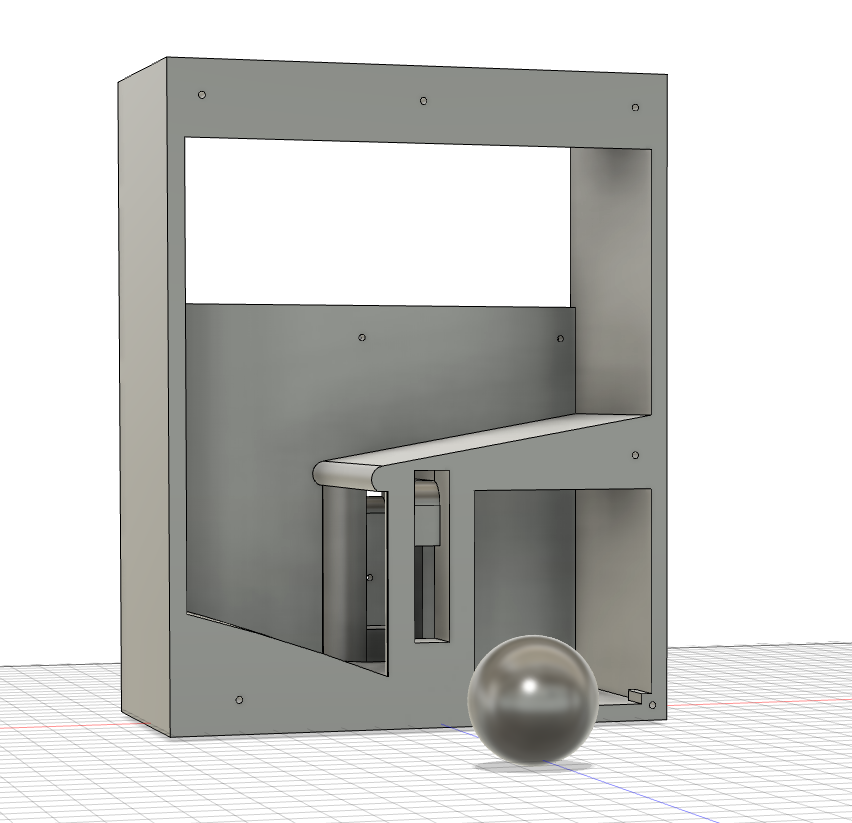
\includegraphics[width=0.3\textwidth]{images/3D/gate_inside.png}
  \caption{Model bramki razem z piłeczką}
  \label{fig:mobile}
\end{figure}

\section{Druk 3D}
Gotowy projekt modelu został przygotowany do druku w programie Cura. Czas druku samej bramki zajął około 30 godzin. Poza bramką wydrukowane zostały również elemnty takie jak tył bramki oraz piłka. W celu odwzorowania ruchu piłki taki jaki występuje podczas gry w piłkarzyki, gabaryty oraz waga piłeczki zostały zbliżone tym dostępnych na rynku (średnica 35 milimetrów oraz około 15 gram wagi). Ze względu na cenę i dostępność wszystkie elementy zostały wydukowane z materiału PLA na drukarce Ender CR20 Pro.

\begin{figure}[h!]
  \centering
    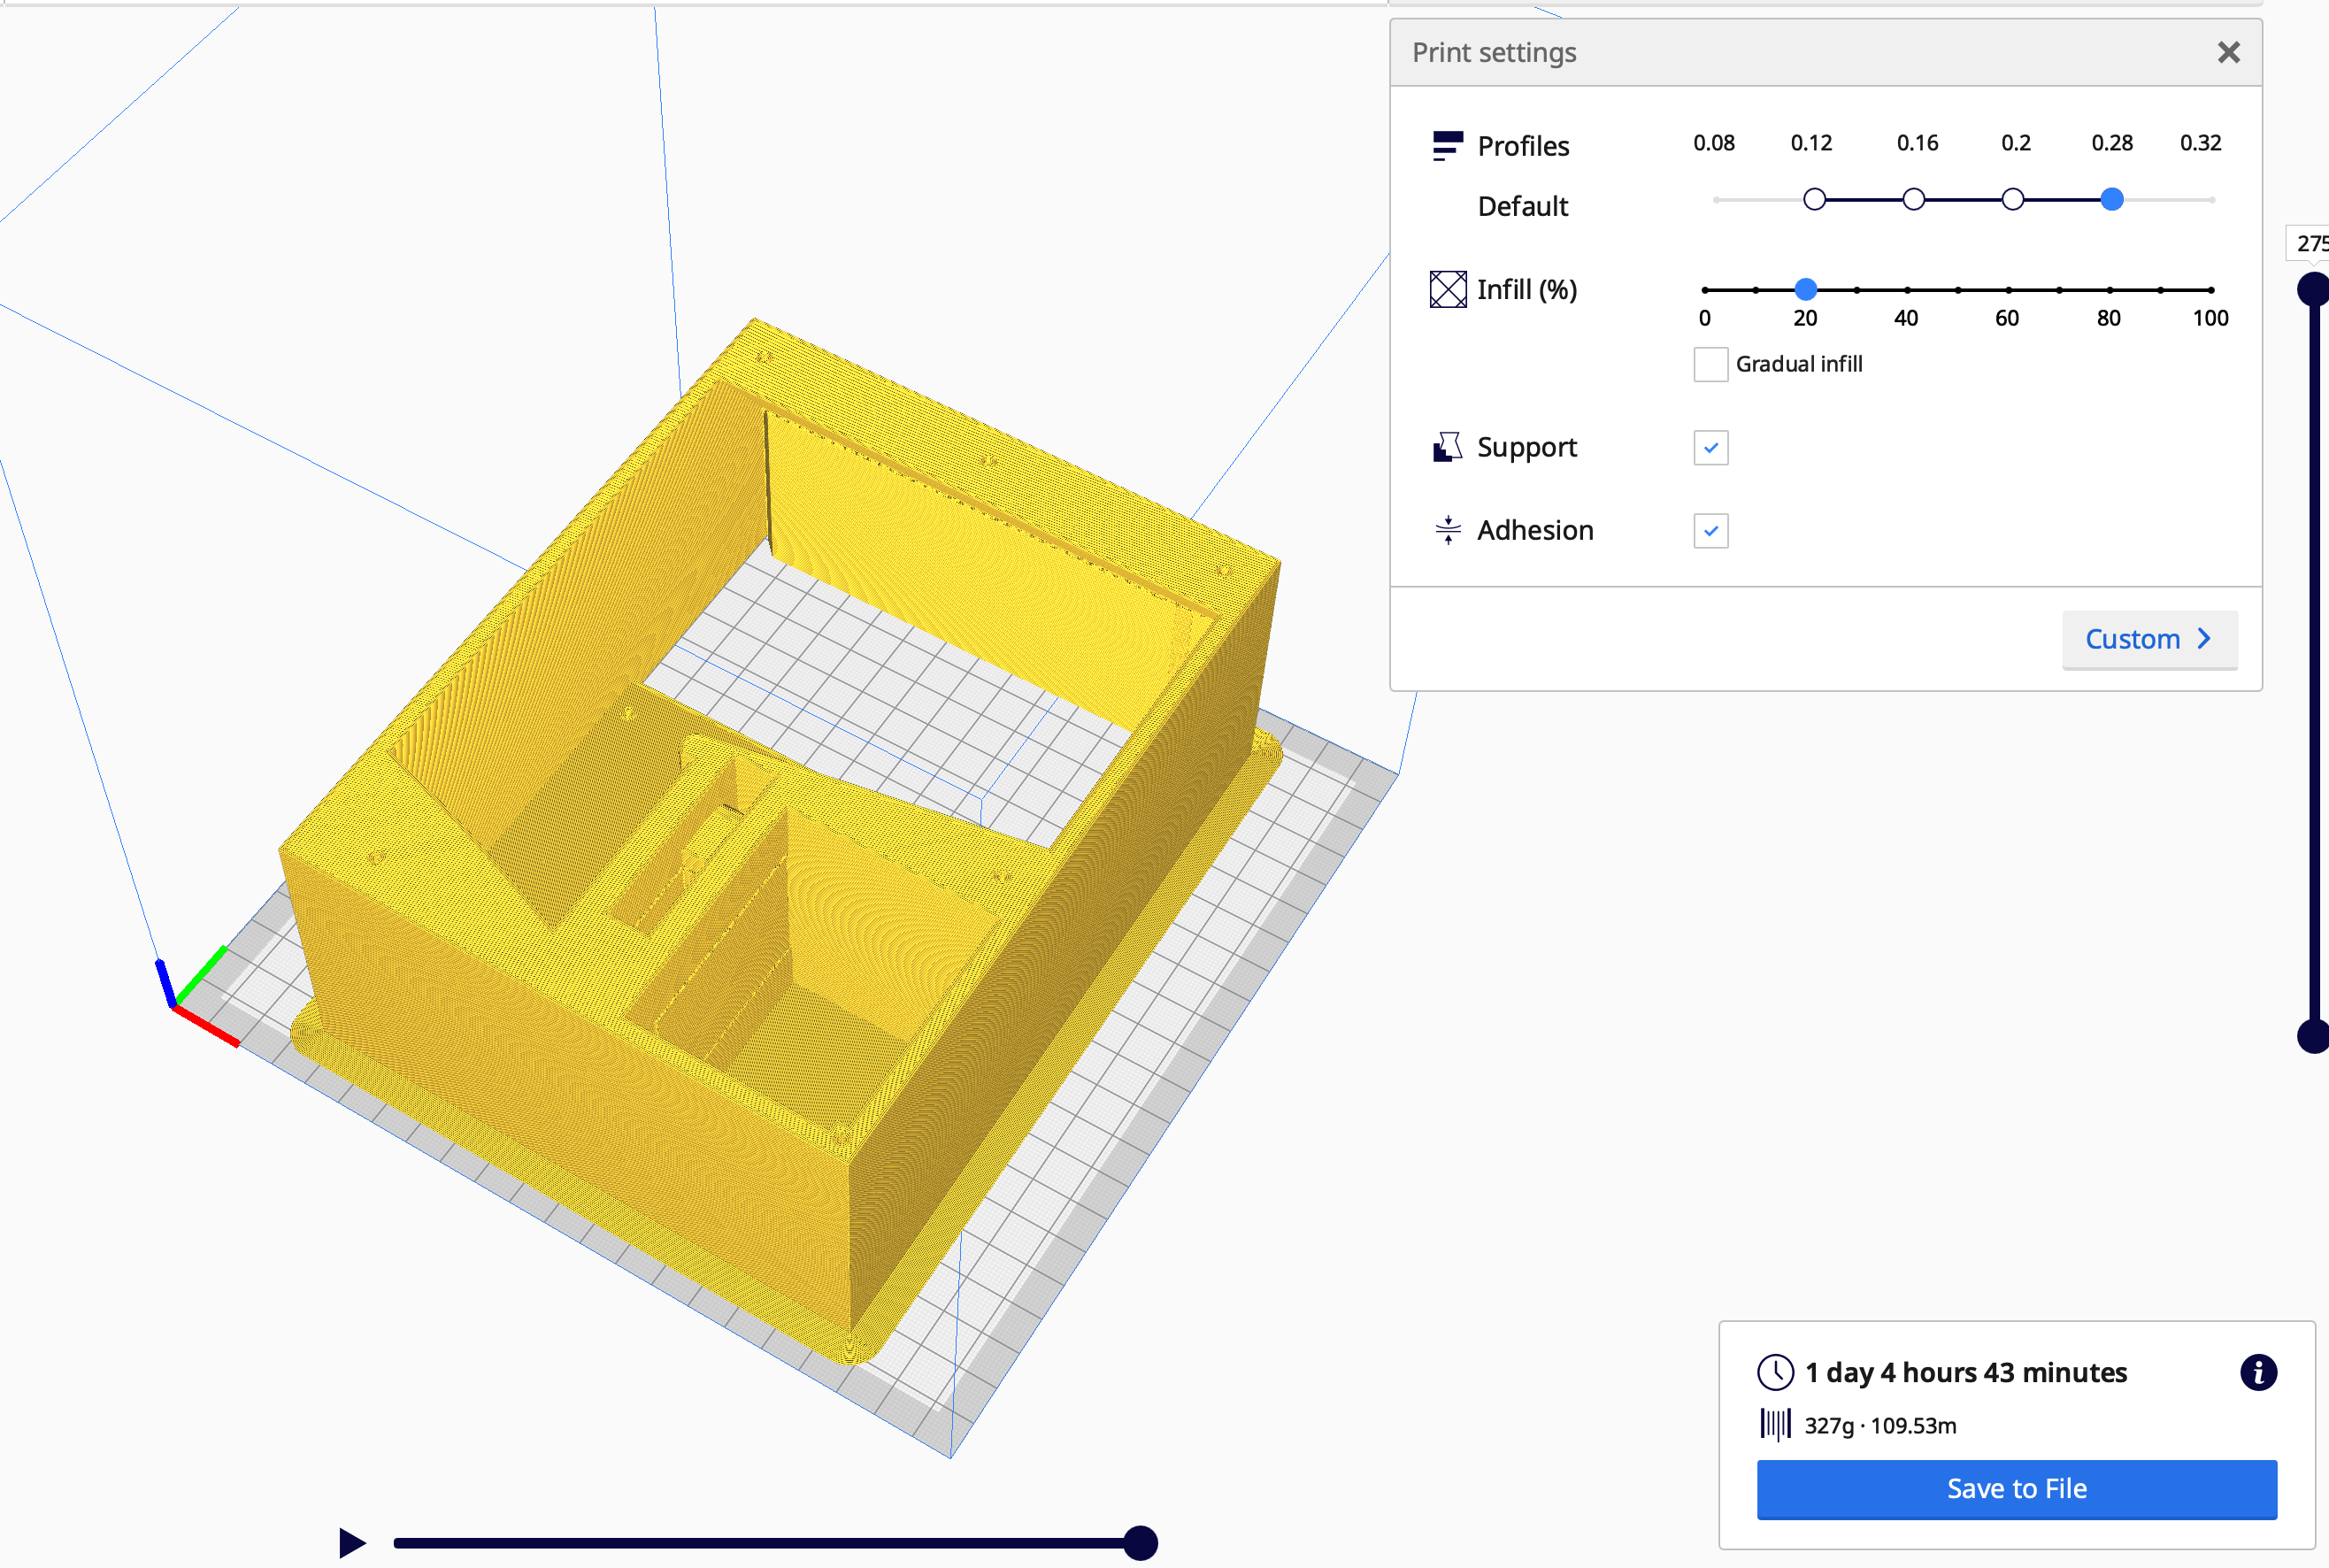
\includegraphics[width=0.5\textwidth]{images/3D/cura_gate.png}
  \caption{Przygotowanie modelu do druku}
  \label{fig:mobile}
\end{figure}

\section{Raspberry}
% https://www.raspberrypi.org/about/
% https://pl.wikipedia.org/wiki/Wej%C5%9Bcie-wyj%C5%9Bcie_og%C3%B3lnego_przeznaczenia
Kolejnym i ostatnim elementem systemu w tym rozdziale jest zastsowane w projekcie Raspberry Pi. Mini komputer, który odpowiada za zarządzanie i komunikacje urzedzęń takich jak kamera, diody czy sensory bramek z resztą systemu. Zaprojektowany i wydany przez brytyjską organizację Raspberry Pi. Alrenatywami podczas wyboru mini komputera były inne wersje Raspberry Pi lub Arduino. Projekt wykorzystuje wersje Raspberry Pi 4B ze względu przez posiadanie przez autora już tego modelu. Urzędzenie te oferuje proste podłączenie kamery zarówno po złączu USB jak i natywny dla Raspberry wejściu kamery. Pozostałe czujniki/diody podłączane są z użyciem GPIO. GPIO oznacza wejście-wyjście ogólnego przeznaczenia (od ang. general-purpose input/output).

Do omawianego narzędzia została podłączona kamera, dwa sensory bramek oraz pięć diod indykujących stan działania stołu. Wykorzystany w projekcie sensor bramki to dokładnie czujnik przerwania wiązki IR o wymiarach 20 x 10 x 8 milimetrów.

\begin{figure}[h!]
  \centering
    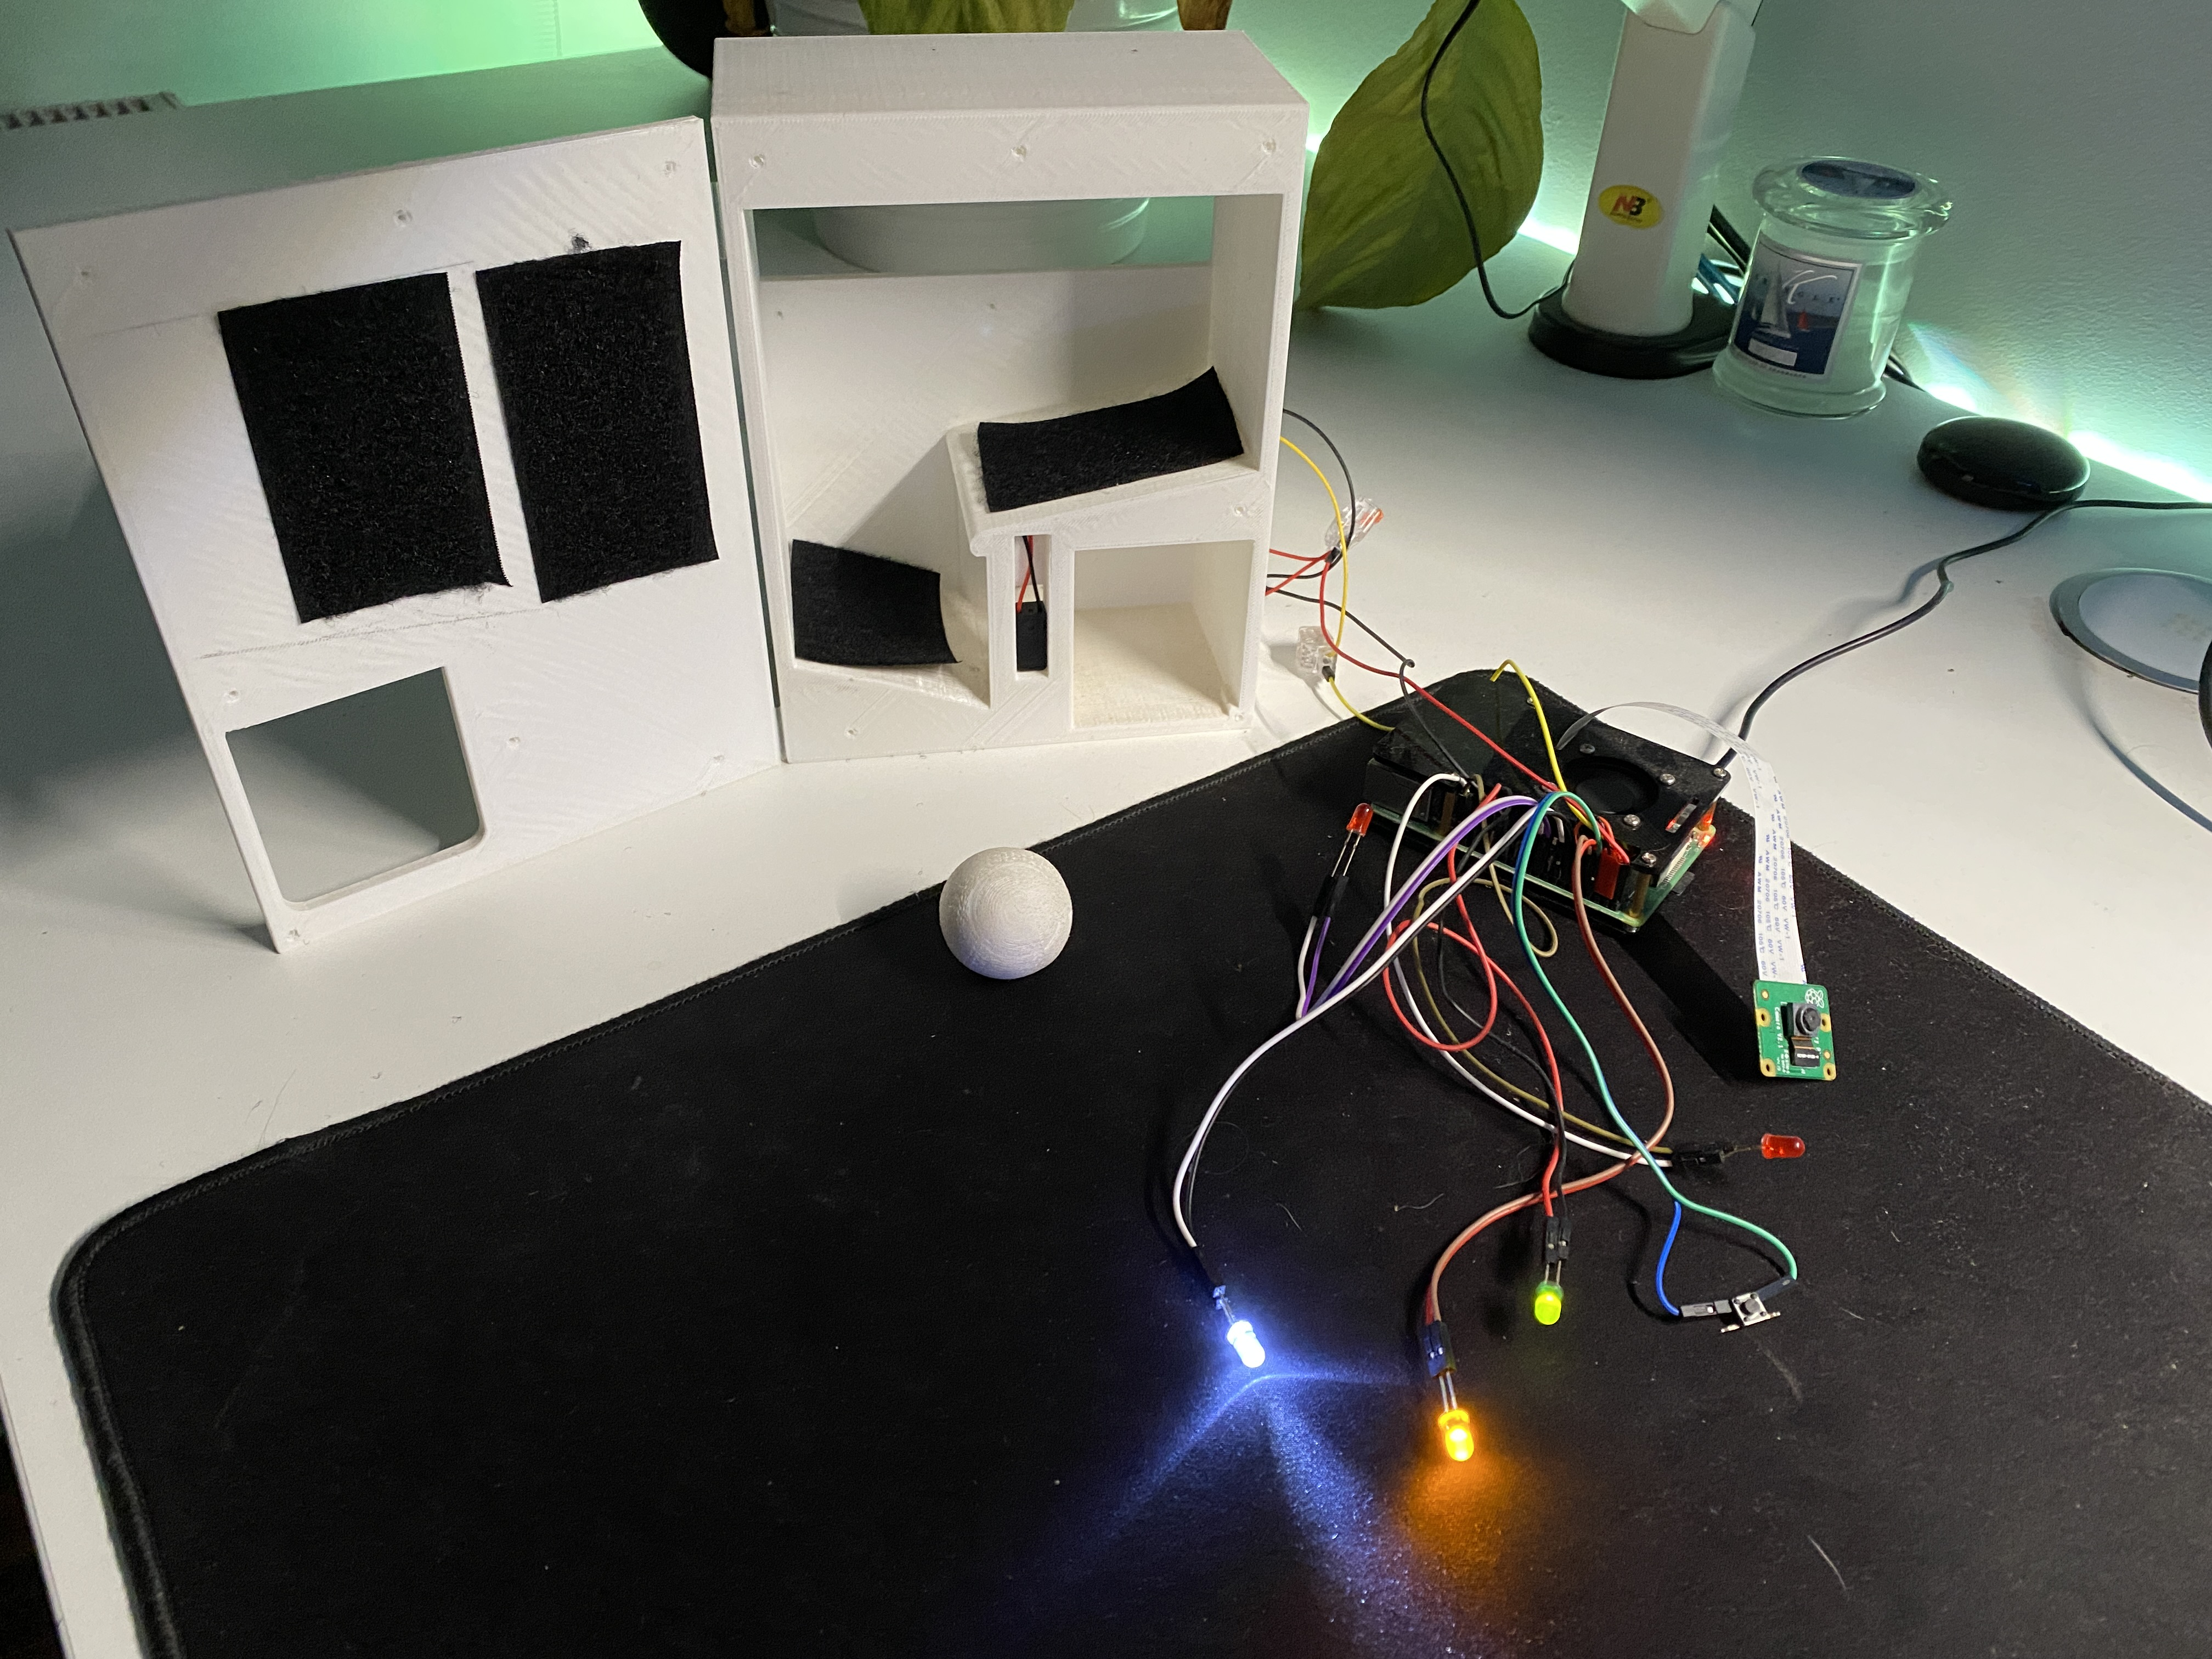
\includegraphics[width=0.5\textwidth]{images/hardware/prototyp-bramki.jpg}
  \caption{Podłączony prototyp bramki}
  \label{fig:mobile}
\end{figure}